\chapter{Proof of Concept}
\label{sec:proof_of_concept}

In this chapter, we present a proof of concept for the fuzzy tuning technique. We will develop a set of linguistic variables and fuzzy rules to predict the optimal configuration parameters for md\_flexible simulations.

\section{Creating the Knowledge Base}

One of the hardest parts of developing a fuzzy system is creating the knowledge base, as it typically requires a very deep understanding of the system to be able to create meaningful rules. However, there also exist methods to use a data-driven approach to create the knowledge base automatically. This is especially useful as those methods don't require any prior expert knowledge about the system. But regardless of the way the knowledge base is created, it is still possible to manually evaluate and adjust the rules to add manual expert knowledge to the system. Using such data-driven methods can be a good starting point for creating a fuzzy system, as it can provide a good initial set of rules that can be further refined by experts.

There are several methods to automatically create and tune fuzzy systems based on data. Some of the most common methods include genetic algorithms \todo{Add references to the methods}, particle swarm optimization, and decision trees.
In this work, we will use a decision tree aproach proposed by Crockett et al.~\cite{CROCKETT20062809} to create the knowledge base for the fuzzy system. This proposed method uses machine learning to first train a classical decision tree on the dataset and then converts the decision tree into a fuzzy decision tree which can then be used to extract the linguistic variables and fuzzy rules.


\subsection{Decision Trees}

Decision trees are very popular machine learning algorithms that are used for classification and regression tasks. They are defined by recursively partitioning the input using axis-parallel splits~\cite{10.5555/2380985}. There are several algorithms to train decision trees, such as ID3, C4.5, CART, and many others, but they all follow the same basic principle of splitting the input space in such a way that the resulting subsets are as pure as possible, thereby minimizing the impurity of the subsets. The impurity of a subset is typically measured using a metric such as the Gini impurity, entropy, or the mean squared error. \todo{Check if this is correct}

Decision trees are known for their interpretability and can be also be easily visualized. An example of a decision tree is shown in Figure~\ref{fig:decisionTreeExample}.
The interpretability of decision trees makes them a good choice for creating the initial knowledge base for a fuzzy system, as it is very easy to understand and refine the rules created by the decision tree with additional expert knowledge.

% Image of a decision tree
\begin{multicols}{2}
    \begin{figure}[H] % [H] for HERE
        \centering
        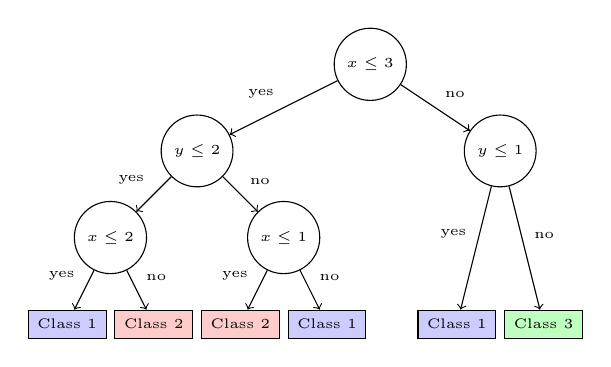
\begin{tikzpicture}[scale=1.1,font=\tiny]
            \node [circle,draw] (A) at (0,0) {$x \leq 3$};
            \node [circle,draw] (B) at (-2,-1) {$y \leq 2$};
            \node [circle,draw] (C) at (1.5,-1) {$y \leq 1$};
            \node [circle,draw] (D) at (-3,-2) {$x \leq 2$};
            \node [circle,draw] (E) at (-1,-2) {$x \leq 1$};

            \node [rectangle,draw,fill=blue!20] (F) at (-3.5,-3) {Class 1};
            \node [rectangle,draw,fill=red!20] (G) at (-2.5,-3) {Class 2};
            \node [rectangle,draw,fill=red!20] (H) at (-1.5,-3) {Class 2};
            \node [rectangle,draw,fill=blue!20] (I) at (-0.5,-3) {Class 1};
            \node [rectangle,draw,fill=blue!20] (J) at (1,-3) {Class 1};
            \node [rectangle,draw,fill=green!25] (K) at (2,-3) {Class 3};

            \draw[->] (A) -- (B) node [midway, left, above left] {yes};
            \draw[->] (A) -- (C) node [midway, right, above right] {no};
            \draw[->] (B) -- (D) node [midway, left, above left] {yes};
            \draw[->] (B) -- (E) node [midway, right, above right] {no};

            \draw[->] (C) -- (J) node [midway, left, above left] {yes};
            \draw[->] (C) -- (K) node [midway, right, above right] {no};

            \draw[->] (D) -- (F) node [midway, left, above left] {yes};
            \draw[->] (D) -- (G) node [midway, right, above right] {no};

            \draw[->] (E) -- (H) node [midway, left, above left] {yes};
            \draw[->] (E) -- (I) node [midway, right, above right] {no};

        \end{tikzpicture}

        \caption[Example Decision Tree]{An example decision tree for a dataset with two features $x$ and $y$. There are three distinct classes in the dataset}
        \label{fig:decisionTreeExample}
    \end{figure}

    \columnbreak    % start next column

    \begin{figure}[H]
        \centering
        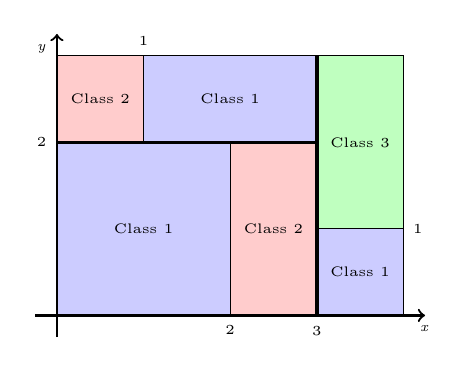
\begin{tikzpicture}[scale=1.1,font=\tiny]

            \draw[fill=red!20] (0,2) -- (1,2) -- (1,3) -- (0,3) -- cycle;

            \draw[fill=blue!20] (1,2) -- (3,2) -- (3,3) -- (1,3) -- cycle;

            \draw[fill=blue!20] (0,0) -- (2,0) -- (2,2) -- (0,2) -- cycle;
            \draw[fill=red!20] (2,0) -- (3,0) -- (3,2) -- (2,2) -- cycle;

            \draw[fill=blue!20] (3,0) -- (4,0) -- (4,1) -- (3,1) -- cycle;
            \draw[fill=green!25] (3,1) -- (4,1) -- (4,3) -- (3,3) -- cycle;

            \draw[->, thick] (-0.25,0) -- (4.25,0) node [below] {\textit{x}};
            \draw[->, thick] (0,-0.25) -- (0,3.25) node [below left] {\textit{y}};

            % decision lines

            \draw[line width=1.5pt,] (3,0) node [below] {3}  -- (3,3) ;
            \draw[line width=1pt] (0,2) node [left] {2} -- (3,2);

            \draw[] (2,0) node [below] {2}-- (2,2);

            \node [above] at (1,3) {1};

            \node [right] at (4,1) {1};

            % area labels
            \node [] at (0.5,2.5) {Class 2};
            \node [] at (2,2.5) {Class 1};

            \node [] at (1,1) {Class 1};
            \node [] at (2.5,1) {Class 2};


            \node [] at (3.5,2) {Class 3};
            \node [] at (3.5,0.5) {Class 1};

        \end{tikzpicture}
        \caption[Decision Boundary]{The decision boundary of the decision tree from Figure~\ref{fig:decisionTreeExample} on $\mathcal{D}=[0,4]\times[0,3]$. }
        \label{fig:decisionBoundaryExample}
    \end{figure}
\end{multicols}



\subsection{Fuzzy Decision Trees}

Fuzzy decision trees are a generalization of classical decision trees that allow for fuzzy logic to be used in the decision-making process. This extension allows to eliminate the crisp decision boundaries of classical decision trees and instead use fuzzy sets at each node of the tree to calculate the contribution of each branch to the final decision. This allows for a more flexible decision-making process that can take into account the uncertainty of the input data and the splits.

Contrary to classical decision trees, which follow a single path from the root to a leaf node, fuzzy decision trees explore all possible paths at the same time and make a final decision by aggregating the results of all paths using fuzzy logic. This is possible, as each node in a fuzzy decision tree can fuzzily assign how much each of its children should contribute to the final decision.

\pgfmathdeclarefunction{sigmoid}{3}{%
    \pgfmathparse{1/(1 + exp(-(#1-#2)*#3))}%
}

\pgfmathdeclarefunction{gaussian}{3}{%
    \pgfmathparse{exp(-((#1-#2)^2)/(2*#3^2))}%
}

\newcommand*\calc[1]{%
    \pgfmathparse{#1}%
    \pgfmathprintnumber{\pgfmathresult}%
}
\pgfplotsset{compat=1.18}

% parameers: xlabel, center
\newcommand{\fuzzyTreeNode}[2]{
    \begin{tikzpicture}
        \begin{axis}%
            [
                title = {Split: $#1 \leq #2$},
                width=4.5cm,
                height=3cm,
                axis lines=center,
                xlabel={#1},
                x label style={at={(axis description cs:0.9,-0.1)},anchor=north},
                ylabel=$\mu$,
                y label style={at={(axis description cs:0.5,1)},anchor=south},
                xmin=-5,
                xmax=5,
                xtick={},
                xticklabels= {},
                ytick={},
                yticklabels={},
                extra x ticks={0},
                extra x tick labels={#2},
                ymax=1,
                samples=50,
                extra y ticks={1},
                every axis plot/.append style={thick}
            ]
            \addplot[red]  {sigmoid(x,0,-1)};
            \addplot[blue] {sigmoid(x,0,1)};
            \node[anchor=center, red] at (axis cs:-2.9,0.6) {$\mu_{\text{#1smaller#2}}$};
            \node[anchor=center, blue] at (axis cs:3.1,0.6) {$\mu_{\text{#1greater#2}}$};
        \end{axis}

    \end{tikzpicture}
}

\newcommand{\fuzzyTreeLeaf}[1]{
    \begin{tikzpicture}
        \begin{axis}%
            [
                title = {Class: #1},
                width=3.25cm,
                height=2.25cm,
                axis lines=center,
                xlabel={$\text{class}$},
                x label style={at={(axis description cs:0.6,-0.3)},anchor=west},
                ylabel=$\mu$,
                y label style={at={(axis description cs:0.5,1)},anchor=south},
                xmin=-5,
                xmax=5,
                xtick={},
                xticklabels= {},
                ytick={},
                yticklabels={},
                extra x ticks={0},
                extra x tick labels={#1},
                ymax=1,
                samples=10,
                extra y ticks={1},
                every axis plot/.append style={thick}
            ]
            \addplot[black]  {gaussian(x,0,1)};
        \end{axis}

    \end{tikzpicture}
}

\begin{figure}[H] % [H] for HERE
    \centering
    \begin{tikzpicture}[scale=2,font=\tiny]

        \node [rectangle,rounded corners,draw,inner sep=2pt] (A) at (0,0) {
            \fuzzyTreeNode{x}{3}
        };

        \node [rectangle,rounded corners,draw,inner sep=2pt] (B) at (-2,-1.75) {
            \fuzzyTreeNode{y}{2}
        };

        \node [rectangle,rounded corners,draw,inner sep=2pt] (C) at (1.5,-1.75) {
            \fuzzyTreeNode{y}{1}
        };

        \node [rectangle,rounded corners,draw,inner sep=2pt] (D) at (-3,-3.5) {
            \fuzzyTreeNode{x}{2}
        };

        \node [rectangle,rounded corners,draw,inner sep=2pt] (E) at (-1,-3.5) {
            \fuzzyTreeNode{x}{1}
        };


        \node [rectangle,rounded corners,draw,inner sep=2pt,fill=blue!20] (F) at (-3.5,-5) {
            \fuzzyTreeLeaf{1}
        };

        \node [rectangle,rounded corners,draw,inner sep=2pt,fill=red!20] (G) at (-2.5,-5) {
            \fuzzyTreeLeaf{2}
        };

        \node [rectangle,rounded corners,draw,inner sep=2pt,fill=red!20] (H) at (-1.5,-5) {
            \fuzzyTreeLeaf{2}
        };

        \node [rectangle,rounded corners,draw,inner sep=2pt,fill=blue!20] (I) at (-0.5,-5) {
            \fuzzyTreeLeaf{1}
        };

        \node [rectangle,rounded corners,draw,inner sep=2pt,fill=blue!20] (J) at (1,-5) {
            \fuzzyTreeLeaf{1}
        };

        \node [rectangle,rounded corners,draw,inner sep=2pt,fill=green!20] (K) at (2,-5) {
            \fuzzyTreeLeaf{3}
        };



        \draw[->] (A) -- (B) node [midway, left, above left] {yes};
        \draw[->] (A) -- (C) node [midway, right, above right] {no};
        \draw[->] (B) -- (D) node [midway, left, above left] {yes};
        \draw[->] (B) -- (E) node [midway, right, above right] {no};

        \draw[->] (C) -- (J) node [midway, left, above left] {yes};
        \draw[->] (C) -- (K) node [midway, right, above right] {no};

        \draw[->] (D) -- (F) node [midway, left, above left] {yes};
        \draw[->] (D) -- (G) node [midway, right, above right] {no};

        \draw[->] (E) -- (H) node [midway, left, above left] {yes};
        \draw[->] (E) -- (I) node [midway, right, above right] {no};
    \end{tikzpicture}

    \caption[Example Fuzzy Decision Tree]{The fuzzy decision tree corresponding created from the decision tree in Figure~\ref{fig:decisionTreeExample}. Each internal node in the fuzzy decision tree uses two \texttt{sigmoid} membership functions (\textcolor{red}{$\mu_{\text{smaller}}$} and \textcolor{blue}{$\mu_{\text{greater}}$} with appropriate parameters) to specify to which degree the comparison is true or false. The leaf nodes use different \texttt{gaussian} membership functions centered around the class value.

        Note that the individual membership functions can be chosen arbitrarily and don't have to be restricted to the ones shown here.}

    \label{fig:fuzzyDecisionTreeExample}
\end{figure}

\subsubsection{Rule Extraction}

Once the fuzzy decision tree has been created, the next step is to extract the fuzzy rules from the tree. This can be done by traversing the tree in a depth-first manner and collecting the correct membership functions for the path along the way. Each connection between two internal nodes in the tree corresponds to a \texttt{AND} operation, while each final connection between an internal node and a leaf node corresponds to an \texttt{IMPLIES} operation.

